% WRFDA overview prepared for 4th east asia WRF tutorial and workshop
% March 2010 
% Autor: Xin Zhang 
% MMM, National Center for Atmospheric Research
% www.mmm.ucar.edu
% email: xinzhang@ucar.edu

\documentclass{beamer}
%\usepackage{pgfpages}
%\pgfpagesuselayout{4 on 1}[a4paper, landscape,border shrink=10mm]
\usepackage{amsmath,amssymb}
\usepackage{times}
\setbeamercovered{dynamic}
\setbeamertemplate{navigation symbols}{}
\usetheme{AnnArbor}
\usepackage{graphics}
\usepackage{eurosym}
\usepackage{tikz}
\usepackage{hyperref}
\usetikzlibrary{shapes,arrows}
\beamersetuncovermixins{\opaqueness<1>{25}}{\opaqueness<2->{15}}
\begin{document}

\title[WRFDA System]{WRF Data Assimilation System Overview}

\author[Xin Zhang et al.]{Xin Zhang \and S. R. Rizvi \and M. Duda \and H. Huang}
\institute[NCAR]{National Center for Atmospheric Research, Boulder, CO USA}
\date{The 5th East Asia WRF Tutorial}
\logo{
\includegraphics[scale=0.13]{ncar_logo}}

% Define block styles
\tikzstyle{minim} = [rectangle, draw, fill=gray!20, rounded corners,
    text width=8em, text centered, node distance=4.4cm, minimum height=2em]
\tikzstyle{runningminim} = [rectangle, draw, fill=green!100, rounded corners,
    text width=8em, text centered, node distance=4.4cm, minimum height=2em]
\tikzstyle{ana} = [rectangle, draw, fill=blue!20, node distance=4.0cm, 
    text width=3.7em, text centered, rounded corners, minimum height=2em]
\tikzstyle{runningana} = [rectangle, draw, fill=green!100, node distance=4.0cm, 
    text width=3.7em, text centered, rounded corners, minimum height=2em]
\tikzstyle{block} = [rectangle, draw, fill=blue!20, node distance=2.1cm, 
    text width=3.7em, text centered, rounded corners, minimum height=2em]
\tikzstyle{runningblock} = [rectangle, draw, fill=green!100, node distance=2.1cm, 
    text width=3.7em, text centered, rounded corners, minimum height=2em]
\tikzstyle{line} = [draw, very thick, color=black!50, -latex']
\tikzstyle{cloud} = [draw, ellipse,fill=red!20, node distance=1.5cm,
    minimum height=1.5em, text width=2.5em, text centered]

\newcommand{\wrfdaFlow}{
    % Place node
    \node [block] (setupFrame) {Setup\\Frame};
    \node [block, right of=setupFrame] (readNml) {Read\\namelist};
    \node [cloud, above of=readNml] (nml) {namelist};
    \node [block, right of=readNml] (setupBg) {Setup\\Background};
    \node [cloud, above of=setupBg] (xb) {$\mathbf{x}^b$};
    \node [block, right of=setupBg] (setupBE) {Setup\\Background\\Error};
    \node [cloud, above of=setupBE] (b0) {$\mathbf{B}$};
    \node [block, right of=setupBE] (setupOb){Setup\\Observations};
    \node [cloud, above of=setupOb] (yo) {$\mathbf{y}$};
    \node [block, below of=setupOb] (calInnov){Calculate\\$\mathbf{y}-H(\mathbf{x}$)};
    \node [minim, left of=calInnov] (minim){Minimize Cost Function};
    \node [ana, left of=minim] (ana){Compute\\Analysis};
    \node [block, below of=ana] (calDia){Calculate\\Diagnostics};
    \node [cloud, below of=calDia] (diagFiles) {Diag. Files};
    \node [block, right of=calDia] (output){Output\\Analysis};
    \node [cloud, below of=output] (xa) {$\mathbf{x}^a$};
    \node [block, right of=output] (tidyUp){Tidy Up};
    % Draw edges
    \path [line] (setupFrame) -- (readNml);
    \path [line] (nml) -- (readNml);
    \path [line] (readNml) -- (setupBg);
    \path [line] (xb) -- (setupBg);
    \path [line] (setupBg) -- (setupBE);
    \path [line] (b0) -- (setupBE);
    \path [line] (setupBE) -- (setupOb);
    \path [line] (yo) -- (setupOb);
    \path [line] (setupOb) -- (calInnov);
    \path [line] (calInnov) -- (minim);
    \path [line] (minim) -- (ana);
    \path [line] (ana) -- (calDia);
    \path [line] (calDia) -- (output);
    \path [line] (calDia) -- (diagFiles);
    \path [line] (output) -- (xa);
    \path [line] (output) -- (tidyUp);
}

\frame{\titlepage}

\begin{frame}[allowframebreaks]
\frametitle{Outline} 
\tableofcontents
\end{frame}

\section{WRFDA in WRF Modeling System}

\begin{frame}
\frametitle{WRFDA in WRF Modeling System}
\begin{center}
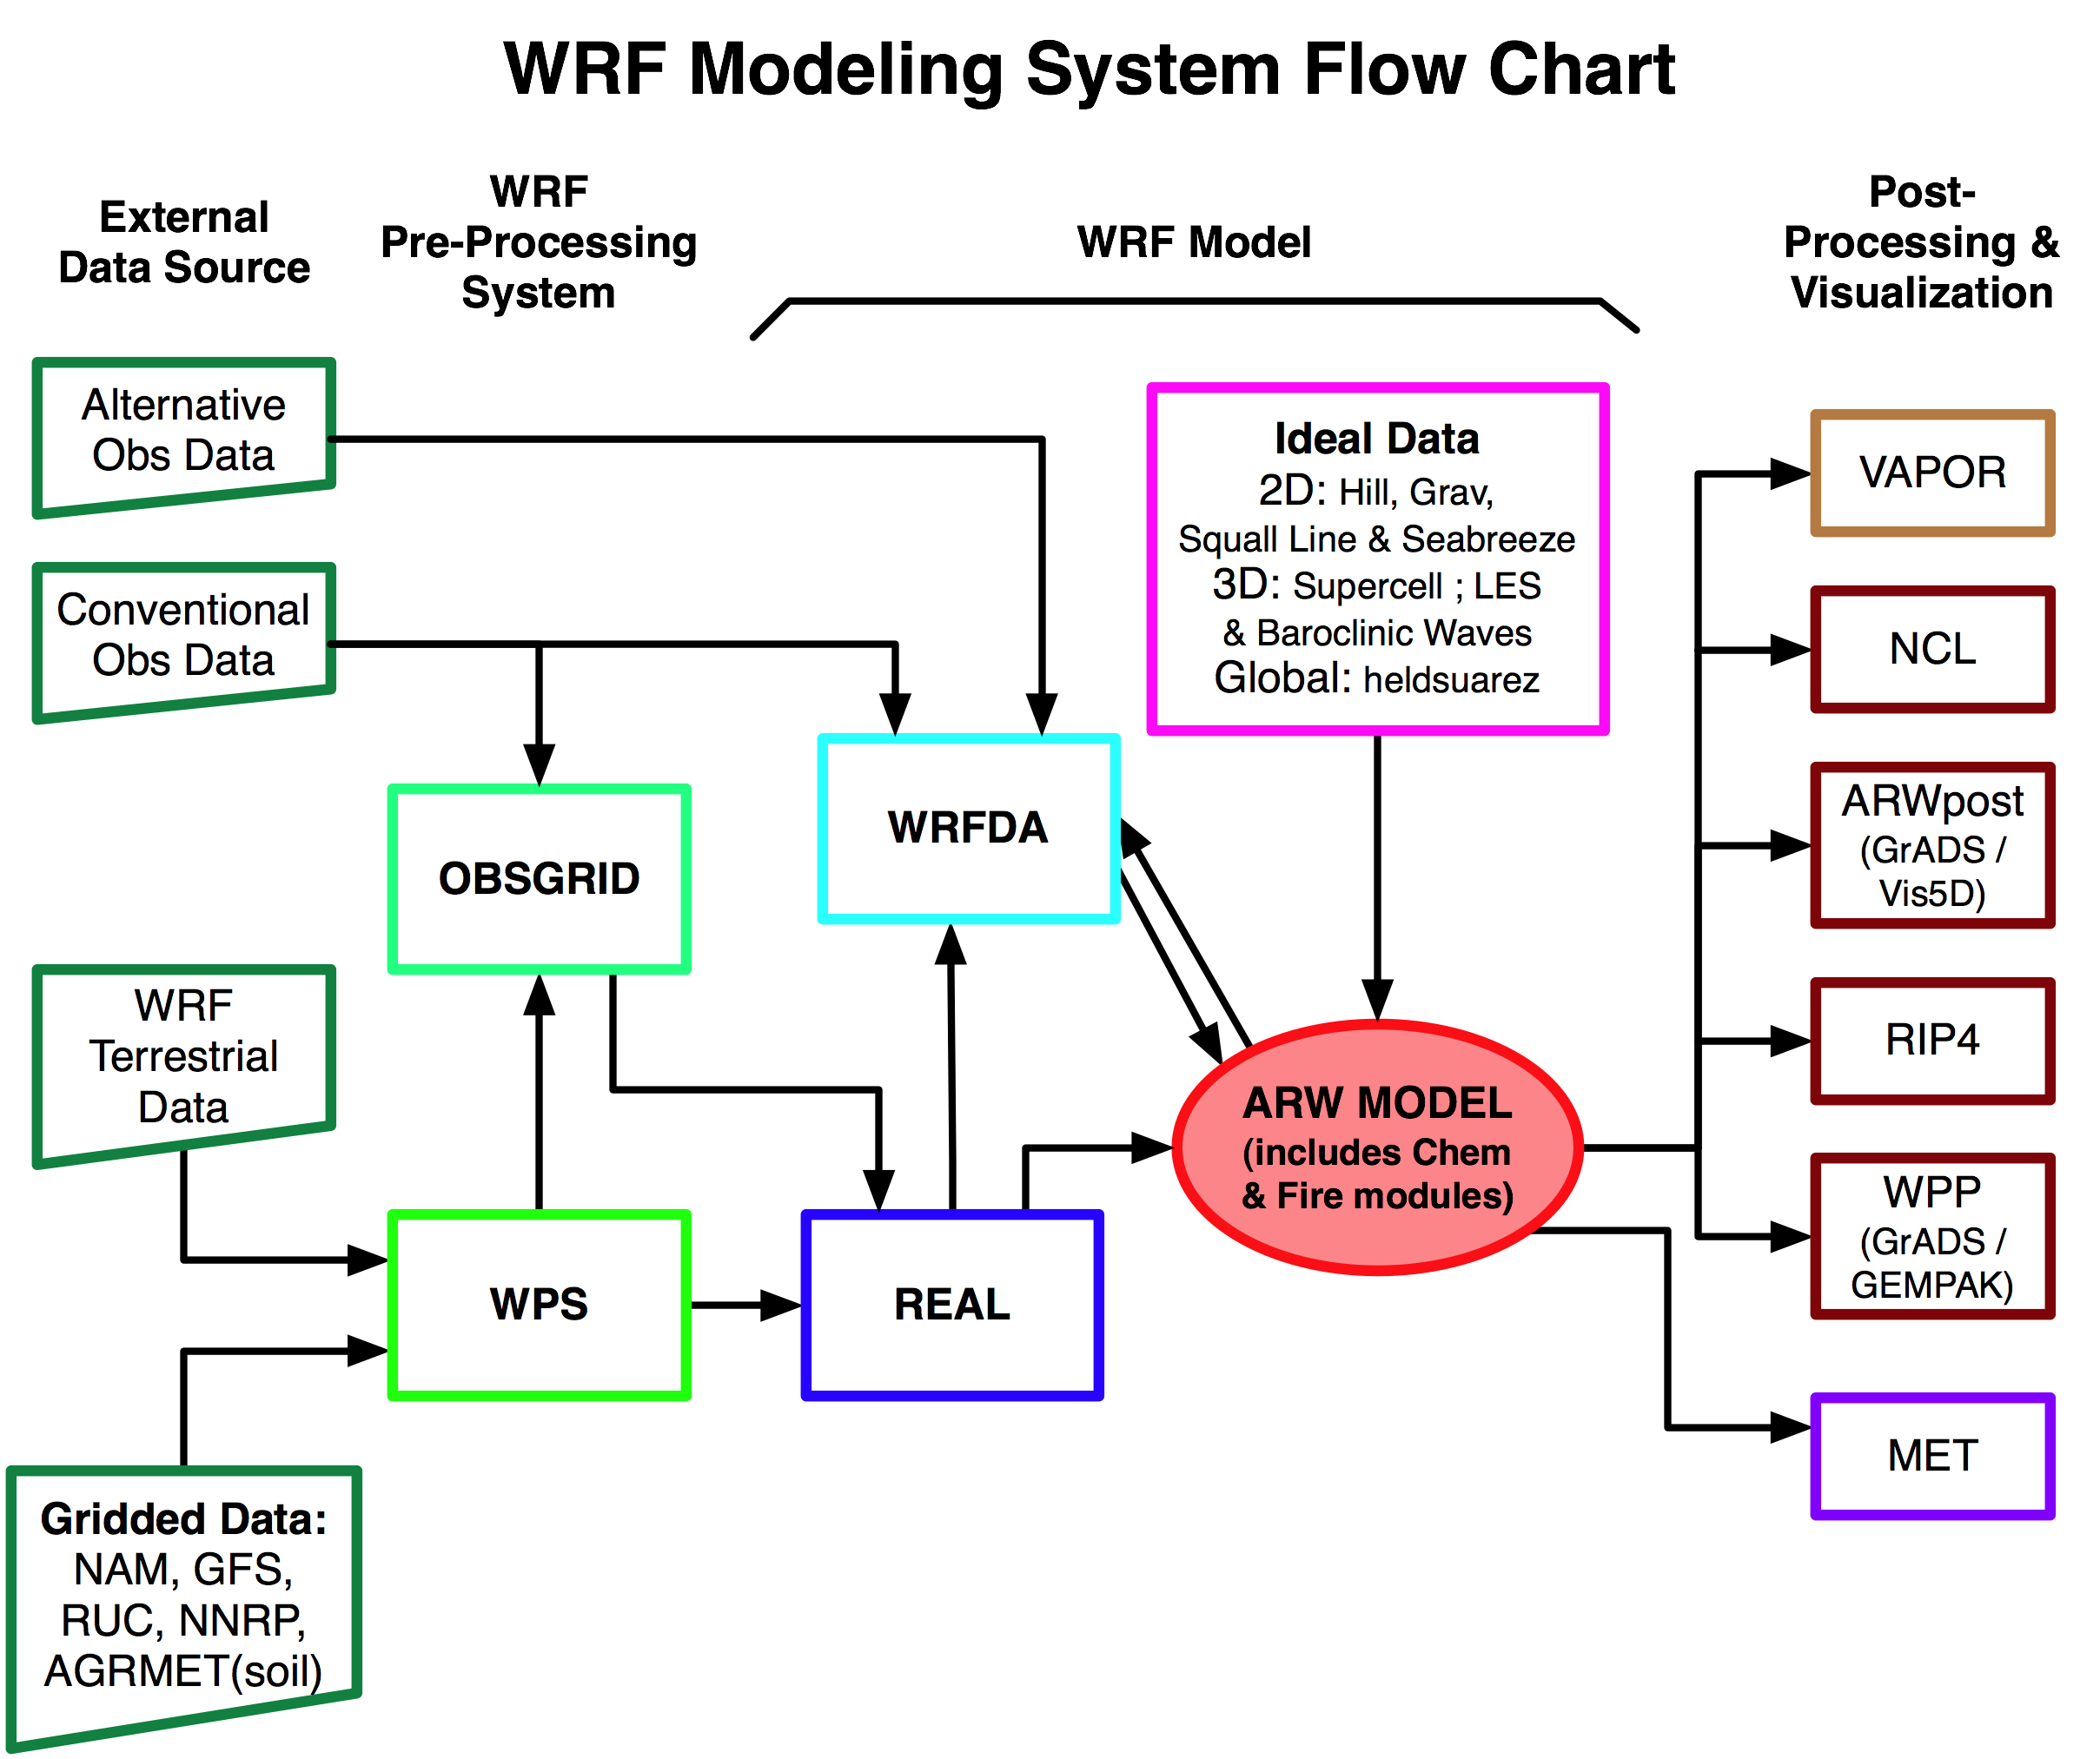
\includegraphics[scale=0.4]{wrfFlowChart}
\end{center}
\end{frame}

\subsection{Prepare the BE}
\begin{frame}
\frametitle{Prepare the BE}
\begin{equation*}
J(\bf{x})=\frac{1}{2}(\bf{x}-\bf{x}^b)^T{\color{red}\bf{B}^{-1}}(\bf{x}-\bf{x}^b)+\frac{1}{2}(\bf{y}-\textsl{H}(\bf{x}))^T\bf{R}^{-1}(\bf{y}-\textsl{H}(\bf{x}))
\end{equation*}
\begin{itemize}
\item Nominally, {\color{red}$\mathbf{B}$} is the background error covariance \pause
\item For initial testing, default background error statistics may
be used \pause 
\begin{itemize}
\item be.dat file (CV option 5) from test case tar file can only be used
with the domain from online tutorial \pause
\item be.dat.cv3 (CV option 3) from source code tar file can be used for
general test domains 
\end{itemize} \pause
\item Ultimately, {\color{red}$\mathbf{B}$} should be specific to the particular
model domain (and season)
\end{itemize}
\end{frame}

\subsection{Prepare the Background}
\begin{frame}
\frametitle{Prepare the Background}
\begin{equation*}
J(\bf{x})=\frac{1}{2}(\bf{x}-{\color{red}\bf{x}^b})^T{\color{blue}\bf{B}^{-1}}(\bf{x}-{\color{red}\bf{x}^b})+\frac{1}{2}(\bf{y}-\textsl{H}(\bf{x}))^T\bf{R}^{-1}(\bf{y}-\textsl{H}(\bf{x}))
\end{equation*}
\begin{itemize}
\item In “cold-start” mode: accomplished by running the
WPS and real programs \pause
\begin{itemize}
\item The background is essentially the wrfinput\_d01 file
\end{itemize} \pause
\item In “cycling” mode: the output of the WRF model \pause
\begin{itemize}
\item WRF can output wrfinput-formatted files used for cycling 
\end{itemize}
\end{itemize}
\end{frame}

\subsection{Prepare the Observations}
\begin{frame}
\frametitle{Prepare the Observations and Assign the Observational Error}
\begin{equation*}
J(\bf{x})=\frac{1}{2}(\bf{x}-{\color{blue}\bf{x}^b})^T{\color{blue}\bf{B}^{-1}}(\bf{x}-{\color{blue}\bf{x}^b})+\frac{1}{2}({\color{red}\bf{y}}-\textsl{H}(\bf{x}))^T{\color{red}\bf{R}^{-1}}({\color{red}\bf{y}}-\textsl{H}(\bf{x}))
\end{equation*}
\begin{itemize}
\item Conventional observation input for WRFDA is supplied through \pause
\begin{itemize}
\item Little\_R format, observation preprocessor, OBSPROC \pause
\item  Prepbufr format data directly \pause
\end{itemize} \pause
\item Observation error covariance also provided by OBSPROC (R is a diagonal matrix) \pause
\item \alert{Separate input file (ASCII) for radar, both reflectivity and radial velocity} \pause
\item \alert{Separate input file for satellite radiances, BUFR format} 
\end{itemize}
\end{frame}

\subsection{Run WRFDA}
\begin{frame}
\frametitle{Run WRFDA}
\begin{equation*}
J(\bf{x})=\frac{1}{2}(\bf{x}-{\color{blue}\bf{x}^b})^T{\color{blue}\bf{B}^{-1}}(\bf{x}-{\color{blue}\bf{x}^b})+\frac{1}{2}({\color{blue}\bf{y}}-\textsl{H}(\bf{x}))^T{\color{blue}\bf{R}^{-1}}({\color{blue}\bf{y}}-\textsl{H}(\bf{x}))
\end{equation*}
\begin{itemize}
\item $H$ is the observational operator, which calculate the counterpart of observations in model space \pause
\item Conjuagate gradient method
\item Try to find a $\mathbf{x}^a$ , which make the $J$ minimal
\end{itemize}
\end{frame}

\subsection{Run UPDATE\_BC}
\begin{frame}
\frametitle{Update Boundary Condition}
\begin{itemize}
\item After creating an analysis, $\bf{x^a}$, we have changed
the initial conditions for the model \pause
\item However, tendencies in wrfbdy\_d01 file are valid for background, $\bf{x^b}$ \pause
\item The update\_bc program adjusts these tendencies
based on the difference $\bf{x^a - x^b}$ \pause
\item Of course, if $\bf{x^a}$ was produced for reasons other
than running WRF, there is probably not a need to
update boundary conditions
\end{itemize}
\end{frame}

\subsection{FAQ}
\begin{frame}
\frametitle{Frequently Asked Question}
\begin{itemize}
\item“Q: What background errors are best for my application?” \pause
\item \alert{A: With gen\_be, create your own once you have run your
system for a few weeks to a month, Implement, tune, and iterate}
\end{itemize}
\end{frame}

\section{WRFDA Implementation}


\subsection{Setup Frame}
\begin{frame}
\frametitle{Setup Frame}
\begin{tikzpicture}[scale=1, node distance = 1.5cm, auto, font=\scriptsize]
\wrfdaFlow
\node [runningblock] (setupFrame) {Setup\\Frame};
\end{tikzpicture}
\end{frame}

\begin{frame}
\frametitle{Setup Frame}
\begin{itemize}
\item Reads grid dimensions from “namelist.input” file \pause
\item Use WRF framework’s distributed memory capability to initialize tile, memory, patch dimensions, etc.
\end{itemize}
\end{frame}

\subsection{Read namelist}
\begin{frame}
\frametitle{Read namelist}
\begin{tikzpicture}[scale=1, node distance = 2.0cm, auto, font=\scriptsize]
\wrfdaFlow
\node [runningblock, right of=setupFrame] (readNml) {Read\\namelist};
\end{tikzpicture}
\end{frame}

\begin{frame}
\frametitle{Read namelist}
\begin{itemize}
\item Reads WRFDA data assimilation options from “namelist.input” file\pause
\item Performs consistency checks between namelist options.
\end{itemize}
\end{frame}

\subsection{Setup Background}
\begin{frame}
\frametitle{Setup Background}
\begin{tikzpicture}[scale=1, node distance = 2.0cm, auto, font=\scriptsize]
\wrfdaFlow
\node [runningblock, right of=readNml] (setupBg) {Setup\\Background};
\end{tikzpicture}
\end{frame}

\begin{frame}
\frametitle{Setup Background}
\begin{itemize}
\item Reads the first-guess file \pause
\item Extracts fields used by WRFDA \pause
\item Creates background FORTRAN 90 derived data type $xb$ etc.
\item Reference :\href{http://www.mmm.ucar.edu/wrf/users/wrfda/technotes.html}{{\bf Online BE Documents}}
\end{itemize}
\end{frame}

\subsection{Setup Background Error}
\begin{frame}
\frametitle{Setup Background Error}
\begin{tikzpicture}[scale=1, node distance = 2.0cm, auto, font=\scriptsize]
\wrfdaFlow
\node [runningblock, right of=setupBg] (setupBE) {Setup\\Background\\Error};
\end{tikzpicture}
\end{frame}

\begin{frame}
\frametitle{Setup Background Error}
\begin{itemize}
\item Reads in background error statistics \pause
\item Extracts necessary quantities – eigenvectors, eigenvalues, lengthscales, regression coefficients, etc.\pause
\item Creates background error FORTRAN 90 derived data type $be$
\end{itemize}
\end{frame}

\subsection{Setup Observations}
\begin{frame}
\frametitle{Setup Observations}
\begin{tikzpicture}[scale=1, node distance = 2.0cm, auto, font=\scriptsize]
\wrfdaFlow
\node [runningblock, right of=setupBE] (setupOb) {Setup\\Observations};
\end{tikzpicture}
\end{frame}

\begin{frame}
\frametitle{Setup Observations}
\begin{itemize}
\item Reads in observations \pause
\item Creates observation FORTRAN 90 derived data type $ob$ \pause
\item Domain and time check
\end{itemize}
\end{frame}

\subsection{Calculate Innovation}
\begin{frame}
\frametitle{Calculate Innovation}
\begin{tikzpicture}[scale=1, node distance = 2.0cm, auto, font=\scriptsize]
\wrfdaFlow
\node [runningblock, below of=setupOb] (calInnov) {Calculate\\$\mathbf{y}-H(\mathbf{x})$};
\end{tikzpicture}
\end{frame}

\begin{frame}
\frametitle{Calculate Innovation}
\begin{itemize}
\item Calculates “model equivalent” of observations through interpolation and change of variable \pause
\item Computes observation minus first guess ($\mathbf{y}-H(\mathbf{x})$) value \pause
\item Creates innovation vector FORTRAN 90 derived data type $iv$
\end{itemize}
\end{frame}

\subsection{Minimization}
\begin{frame}
\frametitle{Minimization}
\begin{tikzpicture}[scale=1, node distance = 2.0cm, auto, font=\scriptsize]
\wrfdaFlow
\node [runningminim, left of=calInnov] (minim) {Minimize\\Cost Function};
\end{tikzpicture}
\end{frame}

\begin{frame}
\frametitle{Minimization}
Use conjugate gradient method \pause
\begin{itemize}
\item Initializes analysis increments to zero \pause
\item Computes cost function (if desired)\pause
\item Computes gradient of cost function \pause
\item Uses cost function and gradient to calculate new value of analysis control variable
\end{itemize}
\end{frame}

\subsection{Compute Analysis}
\begin{frame}
\frametitle{Compute Analysis}
\begin{tikzpicture}[scale=1, node distance = 2.0cm, auto, font=\scriptsize]
\wrfdaFlow
\node [runningana, left of=minim] (ana) {Compute\\Analysis};
\end{tikzpicture}
\end{frame}

\begin{frame}
\frametitle{Compute Analysis}
\begin{itemize}
\item Once WRFDA has found a converged control variable, convert control variable to model space analysis increments \pause
\item Calculate:\\ 
            analysis = first-guess + analysis increment \pause
\item Performs consistency checks, e.g., remove negative humidity etc. \pause 
\item Optionally, do outer loop
\end{itemize}
\end{frame}

\subsection{Calculate Diagnostics}
\begin{frame}
\frametitle{Calculate Diagnostics}
\begin{tikzpicture}[scale=1, node distance = 2.0cm, auto, font=\scriptsize]
\wrfdaFlow
\node [runningblock, below of=ana] (calDia) {Caculate\\Diagnostics};
\end{tikzpicture}
\end{frame}

\begin{frame}
\frametitle{Calculate Diagnostics}
\begin{itemize}
\item Output $\mathbf{y}-H(\mathbf{x}^b)$, $\mathbf{y}-H(\mathbf{x}^a)$ statistics for all observation types and variables \pause
\item Compute $\mathbf{x}^a-\mathbf{x}^b$ (analysis increment) statistics for all model variables and levels \pause
\item Statistics include minimum, maximum (and their locations), mean and standard deviation.
\end{itemize}
\end{frame}

\subsection{Output Analysis}
\begin{frame}
\frametitle{Output Analysis}
\begin{tikzpicture}[scale=1, node distance = 2.0cm, auto, font=\scriptsize]
\wrfdaFlow
\node [runningblock, right of=calDia] (output) {Output\\Analysis};
\end{tikzpicture}
\end{frame}

\begin{frame}
\frametitle{Output Analysis}
\begin{itemize}
\item Outputs analysis in native model format.
\end{itemize}
\end{frame}

\subsection{Tidy Up}

\begin{frame}
\frametitle{Tidy Up}
\begin{tikzpicture}[scale=0.5, node distance = 2.5cm, auto, font=\scriptsize]
\wrfdaFlow
\node [runningblock, right of=output] (tidyUp) {Tidy\\Up};
\end{tikzpicture}
\end{frame}

\begin{frame}
\frametitle{Tidy Up}
\begin{itemize}
\item Deallocate dynamically-allocated arrays, structures, etc.\pause
\item Timing information \pause
\item Clean end to WRFDA
\end{itemize}
\end{frame}

\section{WRFDA Software}
\subsection{WRFDA Software Framework}
\begin{frame}
\frametitle{Use of the WRF Software Framework} 
\begin{center} 
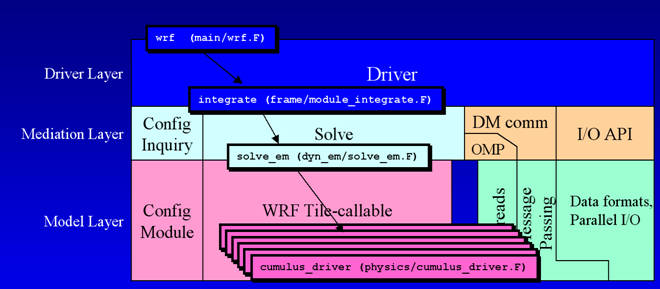
\includegraphics[scale=0.4]{wrfSoftFrame}
\end{center}\pause
\begin{itemize}
\item WRFDA relies on the WRF Software framework for \pause
\begin{itemize}
\item Distributed memory parallelism (halo exchanges, etc.) \pause
\item Input/Output of first guess and analysis files \pause
\item Parallel transposes \pause
\end{itemize} \pause
\item  WRFDA also uses \pause
\begin{itemize}
\item The WRF Registry mechanism to handle definitions of fields, halos, and transposes \pause
\item The WRF build system (clean, configure, compile)
\end{itemize}
\end{itemize}
\end{frame}

\subsection{WRFDA Code Organization}
\begin{frame}
\frametitle{WRFDA Code Organization}
\begin{columns}[c]
\column{5cm}
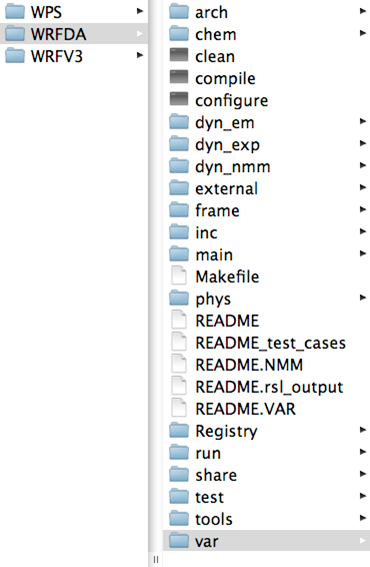
\includegraphics[scale=0.4]{wrfdaCode}
\column{7cm}
Besides the directories for WRF, the WRFDA tar file contains a “var” directory, which holds all of the WRFDA code
\end{columns}
\end{frame}

\begin{frame}
\frametitle{WRFDA Code Organization}
\begin{columns}[c]
\column{5cm}
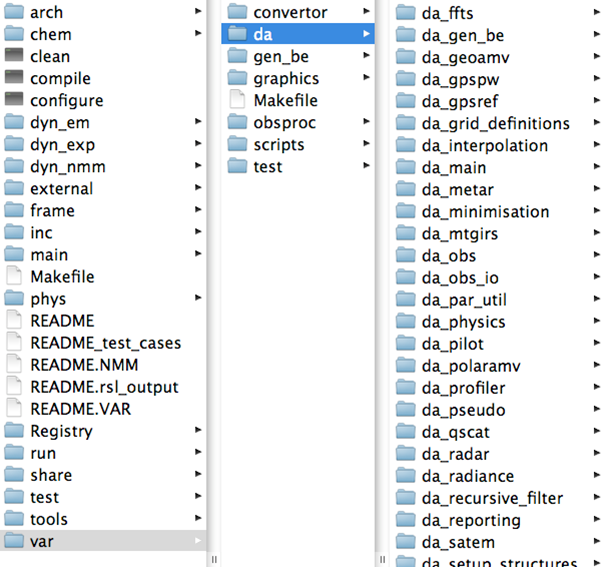
\includegraphics[scale=0.4]{wrfdaCode2}
\column{3cm}
Generally, each subdirectory of “da” contains a Fortran module with the same name
\end{columns}
\end{frame}

\begin{frame}
\frametitle{WRFDA Code Organization}
\begin{columns}[c, totalwidth=12cm]
\column{6cm}
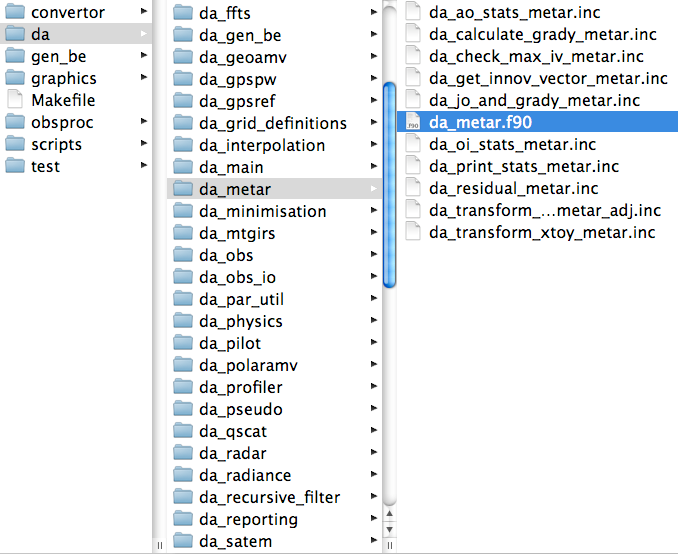
\includegraphics[scale=0.4]{wrfdaCode3}
\column{4.5cm}
\begin{itemize}
\item da\_metar.f90 contains a Fortran module
\item Each .inc file corresponds to a subroutine within the module
\end{itemize}
\end{columns}
\end{frame}

\subsection{Online WRFDA Resources}
\begin{frame}
\frametitle{WRFDA Users' Home Page}
WRFDA has a dedicated page, similar to the ARW Users’ page: \href{http://www.mmm.ucar.edu/wrf/users/wrfda/}{{\bf WRFDA User PAge}}
\begin{center}
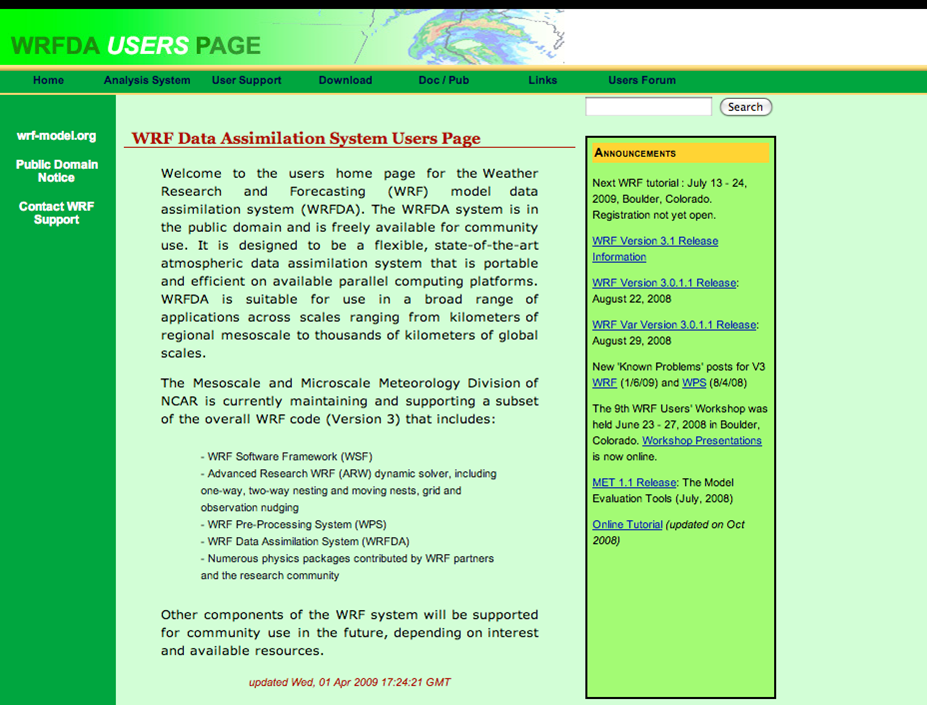
\includegraphics[scale=0.4]{wrfdaHomePage}
\end{center}
\end{frame}

\begin{frame}
\frametitle{Online Resources}
From the WRFDA page, one can access:
\begin{columns}[c, totalwidth=12cm]
\column{6cm}
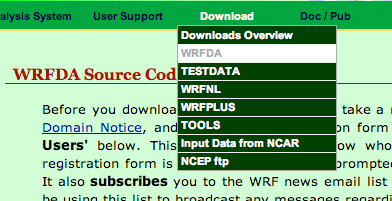
\includegraphics[scale=0.4]{wrfdaDownload}
\column{6cm}
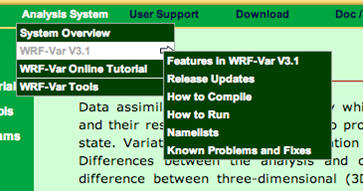
\includegraphics[scale=0.4]{wrfdaSystem}
\end{columns}
\begin{center}
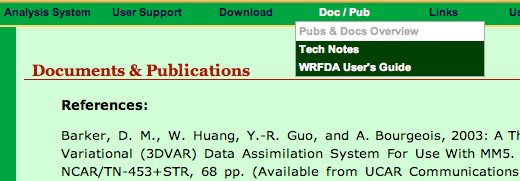
\includegraphics[scale=0.4]{wrfdaDocPub}
\end{center}
\end{frame}

\section{Question}
\begin{frame}
\frametitle{Question?}
\begin{center}
Questions and Comments ?
\end{center}
\end{frame}
\end{document}
